\PassOptionsToPackage{square,numbers}{natbib}
\documentclass{article}


% if you need to pass options to natbib, use, e.g.:
%     \PassOptionsToPackage{numbers, compress}{natbib}
% before loading neurips_2023


% ready for submission
\usepackage[final]{neurips_2023}


% to compile a preprint version, e.g., for submission to arXiv, add add the
% [preprint] option:
%     \usepackage[preprint]{neurips_2023}


% to compile a camera-ready version, add the [final] option, e.g.:
%     \usepackage[final]{neurips_2023}


% to avoid loading the natbib package, add option nonatbib:
%    \usepackage[nonatbib]{neurips_2023}


\usepackage[utf8]{inputenc} % allow utf-8 input
\usepackage[T1]{fontenc}    % use 8-bit T1 fonts
\usepackage{hyperref}       % hyperlinks
\usepackage{url}            % simple URL typesetting
\usepackage{booktabs}       % professional-quality tables
\usepackage{amsfonts}       % blackboard math symbols
\usepackage{nicefrac}       % compact symbols for 1/2, etc.
\usepackage{microtype}      % microtypography
\usepackage{xcolor}         % colors

\usepackage{amsmath}
\usepackage{listings}
\usepackage{graphicx}
\usepackage{placeins}

\definecolor{codegreen}{rgb}{0,0.6,0}
\definecolor{codegray}{rgb}{0.5,0.5,0.5}
\definecolor{codepurple}{rgb}{0.58,0,0.82}
\definecolor{backcolour}{rgb}{0.95,0.95,0.92}

\bibliographystyle{abbrvnat}

\lstdefinestyle{mystyle}{
    backgroundcolor=\color{backcolour},   
    commentstyle=\color{codegreen},
    keywordstyle=\color{magenta},
    numberstyle=\tiny\color{codegray},
    stringstyle=\color{codepurple},
    basicstyle=\footnotesize,
    breakatwhitespace=false,         
    breaklines=true,                 
    captionpos=b,                    
    keepspaces=true,                 
    numbers=left,                    
    numbersep=5pt,                  
    showspaces=false,                
    showstringspaces=false,
    showtabs=false,                  
    tabsize=2,
    frame=single
}
\lstset{style=mystyle}
\lstset{language=Python}

\title{ECE 174 Project 1 Report}


% The \author macro works with any number of authors. There are two commands
% used to separate the names and addresses of multiple authors: \And and \AND.
%
% Using \And between authors leaves it to LaTeX to determine where to break the
% lines. Using \AND forces a line break at that point. So, if LaTeX puts 3 of 4
% authors names on the first line, and the last on the second line, try using
% \AND instead of \And before the third author name.


\author{Pranav Reddy
% \thanks{Use footnote for providing further information
%     about author (webpage, alternative address)---\emph{not} for acknowledging
%     funding agencies.} 
\\
  University of California, San Diego\\
  \texttt{p3reddy@ucsd.edu} \\
  % examples of more authors
  % \And
  % Coauthor \\
  % Affiliation \\
  % Address \\
  % \texttt{email} \\
  % \AND
  % Coauthor \\
  % Affiliation \\
  % Address \\
  % \texttt{email} \\
  % \And
  % Coauthor \\
  % Affiliation \\
  % Address \\
  % \texttt{email} \\
  % \And
  % Coauthor \\
  % Affiliation \\
  % Address \\
  % \texttt{email} \\
}


\begin{document}


\maketitle


\begin{abstract}
  We built the multi-class classifiers as specificed by the writeup.
  In the first part, we construct the binary classifier and use that to build a one-versus-all classifier and a one-versus-one classifier.
  We note that the one-versus-one classifier has markedly better performance, but also takes much longer to train as well and is in general much larger.
  In the second part we utilize four randomized feature mappings: identity, sigmoid, sinusoid, and ReLU, and compare the performance of each on both classifiers.
  We find that the randomized feature mappings produce better performance with both types of classifiers, but do add to the training time.
\end{abstract}


\section{Least Squares Classifier}


In this section we develop an explanation of our code and the theory behind the classifier.

\subsection{Building the Binary Classifier}

We want to form the normal equations from the minimization problem that we were given.
We are given the following least squares problem.
\begin{equation}\label{original-problem}
    \min_{\beta,\alpha} \sum_{i=1}^{N}{(y_i - \beta^\top \mathbf{x}_i + \alpha)}^2
\end{equation}
Then, we can format~\ref{original-problem} as 
\begin{align*}
    \min_{\beta,\alpha} \left\|
        \begin{bmatrix}
        y_1 - \beta^\top \mathbf{x}_1 + \alpha \\
        \vdots\\
        y_N - \beta^\top \mathbf{x}_N + \alpha
    \end{bmatrix}\right\|^2 &= \min_{\beta,\alpha} \left\|\mathbf{y} - 
    \begin{bmatrix}
        \beta^\top \mathbf{x}_1 + \alpha \\
        \vdots\\
        \beta^\top \mathbf{x}_N + \alpha
    \end{bmatrix}\right\|^2 \\
    &= \min_{\beta,\alpha} \left\|\mathbf{y} - 
    \begin{bmatrix}
        \mathbf{x}_1^\top\beta + \alpha \\
        \vdots\\
        \mathbf{x}_N^\top\beta + \alpha
    \end{bmatrix}\right\|^2 \\
    &= \min_{\beta,\alpha} \left\|\mathbf{y} - 
    \begin{bmatrix}
        1 & \mathbf{x}_1^\top \\
        \vdots&\vdots\\
        1 & \mathbf{x}_N^\top
    \end{bmatrix} \begin{bmatrix}
        \alpha \\ \beta
    \end{bmatrix}\right\|^2.\\
\end{align*}
By relabeling the variables in the last equation, we obtain the normal equations
\begin{equation}\label{normal-equations}
    \begin{bmatrix}
        1 & \mathbf{x}_1^\top \\
        \vdots&\vdots\\
        1 & \mathbf{x}_N^\top
    \end{bmatrix}^\top\mathbf{y} = \begin{bmatrix}
        1 & \mathbf{x}_1^\top \\
        \vdots&\vdots\\
        1 & \mathbf{x}_N^\top
    \end{bmatrix}^\top\begin{bmatrix}
        1 & \mathbf{x}_1^\top \\
        \vdots&\vdots\\
        1 & \mathbf{x}_N^\top
    \end{bmatrix}\begin{bmatrix}
        \alpha \\ \beta
    \end{bmatrix}
\end{equation}
For brevity we will write this as 
\begin{equation}\label{normal-equations-simple}
        X^\top\mathbf{y} = X^\top X\theta
\end{equation}
where $\theta$ in~\ref{normal-equations-simple} provides the optimal $\alpha$ and $\beta$ for~\ref{original-problem}.

% ----------------------------------------------------------------------------------------------------------------------------------------------------------------------------------------------
\subsection{One-Versus-All Classifier}
The code implementing all the classifiers is contained in a GitHub repository that is linked in the references.
For speed, we first precompute ${(X^\top X)}^\dag X^\top$ and the multiply by every binary relabeling for speed.
\begin{lstlisting}[frame=single,language=Python, numbers=left, breaklines]
    XTX = np.matmul(trainX.transpose(), trainX)
    XTX_pinv = np.linalg.pinv(XTX)
    XTX_pinv_XT = np.matmul(XTX_pinv,trainX.transpose())

    labels = np.arange(0, 10)

    one_vs_all_model = []
    for i in range(len(labels)):
        binaryY = np.copy(trainY)
        binaryY[binaryY != labels[i]] = -1
        binaryY[binaryY == labels[i]] = 1
        
        one_vs_all_model.append(np.matmul(XTX_pinv_XT,binaryY))
    one_vs_all_model=np.concatenate(one_vs_all_model,axis=1)
\end{lstlisting}
For convenience, we stack the 10 binary classifiers into a single matrix, so that we can simply using matrix multiplication to generate predictions for the data.

\subsubsection{Error Analysis}

\FloatBarrier

\begin{figure}[h!]
    \centering
    \begin{minipage}{0.5\textwidth}
        \centering
        \includegraphics[width=\textwidth]{images/one_vs_all_train_confusion_matrix.eps}
        \caption{Confusion matrix for the training data.}
    \end{minipage}\hfill
    \begin{minipage}{0.5\textwidth}
        \centering
        \includegraphics[width=\textwidth]{images/one_vs_all_test_confusion_matrix.eps}
        \caption{Confusion matrix for the test data.}
    \end{minipage}
\end{figure}
We can see from the confusion matrix that the one-versus-all classifier has solid performance overall but confuses similar looking digits.
The most common error was predicting 1 when the true answer was 8.
On the other hand, 0 was very easily recognized, and 1 had the fewest false negatives.

For the test data performance, we see that the classifier performs well on the test data, even having a slight improvement in performance.
The most common error was predicting 4 when the true answer was 9, and once again the model confuses similar looking digits, such as 3 and 5 or 7 and 9.
Again, 0 was very easily recognized, and 1 had the fewest false negatives.

\FloatBarrier
% ------------------------------------------------------------------------------------------------------------------------------------------------------------------------------------------------------------------
\subsection{One-Versus-One Classifier}
For the one-versus-one classifier, we arrange the $\binom{K}{2}$ classifiers in a 3D array in the following code.
\begin{lstlisting}[frame=single,language=Python, numbers=left, breaklines]
    one_vs_one_model = np.empty((10,10,trainX.shape[1]))

    for i in range(len(labels)):
        for j in range(i+1, len(labels)):
            mask = ((trainY[:,0] == labels[i]) | (trainY[:,0] == labels[j]))
            filtered_Y = trainY[mask]
            filtered_X = trainX[mask]

            filtered_Y[filtered_Y == labels[j]] = -1
            filtered_Y[filtered_Y == labels[i]] = 1
            model_ij = np.matmul(np.matmul(np.linalg.pinv(np.matmul(filtered_X.transpose(),filtered_X)),filtered_X.transpose()),filtered_Y)
            one_vs_one_model[i,j,:] = model_ij[:,0]
\end{lstlisting}

\subsubsection{Error Analysis}

\FloatBarrier

\begin{figure}[h!]
    \centering
    \begin{minipage}{0.5\textwidth}
        \centering
        \includegraphics[width=\textwidth]{images/one_vs_one_train_confusion_matrix.eps}
        \caption{Confusion matrix for the training data.}
    \end{minipage}\hfill
    \begin{minipage}{0.5\textwidth}
        
        \centering
        \includegraphics[width=\textwidth]{images/one_vs_one_test_confusion_matrix.eps}
        \caption{Confusion matrix for the test data.}
    \end{minipage}
\end{figure}
We see that the one-versus-one classifier has improved performance on the training data when compared to the one-versus-all classifier.
The most common error was predicting 1 when the true answer was 8, and once again the model confuses similar looking digits, such as 3 and 5 or 7 and 9.
Again, 0 was very easily recognized, and 1 had the fewest false negatives.

The performance on the test data is slightly worse.
The most common error was predicting 4 when the true answer was 9, and once again the model confuses similar looking digits, such as 3 and 5 or 7 and 9.
Again, 0 was very easily recognized, and 1 had the fewest false negatives.

Overall, we can see that the one-versus-one classifier is a definite improvement over the one-versus-all classifier, but still makes very similar mistakes and errors.
\FloatBarrier
% --------------------------------------------------------------------------------------------------------------------------------------------------------------------------
\section{Randomized Feature Least Squares Classifier}
\subsection{One-Versus-All Classifier}
\subsubsection{One-Versus-All Classifier Implementation}
I implemented the randomized feature mappings with the following Python code:
The functions take in randomized matrices $W$ and $b$ and apply the given mappings to the sum.
\begin{lstlisting}
    def identity(x, W, b):
        n = (x.shape)[0]
        return np.hstack((np.ones((n,1)), np.matmul(x, W)+b[:n, :W.shape[1]]))
    def sin(x, W, b):
        n = (x.shape)[0]
        x = np.matmul(x, W)+b[:n, :W.shape[1]]
        x = np.sin(2 * np.pi * x / 180)
        return np.hstack((np.ones((n,1)), x))
    def relu(x, W, b):
        n = (x.shape)[0]
        x = np.matmul(x, W)+b[:n, :W.shape[1]]
        x = x * (x > 0)
        return np.hstack((np.ones((n,1)), x))
    def sigmoid(x, W, b):
        n = (x.shape)[0]
        x = np.matmul(x, W)+b[:n, :W.shape[1]]
        x = scipy.special.expit(x)
        return np.hstack((np.ones((n,1)), x))
\end{lstlisting}

After that, I extracted the code to create the classifier into a few different methods, shown here:
\begin{lstlisting}
    def create_model(x, y, labels):
        XTX = np.matmul(x.transpose(), x)
        XTX_pinv = np.linalg.pinv(XTX)
        XTX_pinv_XT = np.matmul(XTX_pinv,x.transpose())
        model = []
        for i in range(len(labels)):
            binary = np.copy(y)
            binary[binary != labels[i]] = -1
            binary[binary == labels[i]] = 1
            model.append(np.matmul(XTX_pinv_XT,binary))
        model=np.concatenate(model,axis=1)
        return model

    def create_model_error_analysis(trueY, predictions):
        error = 0
        for i in range(len(predictions)):
            if(predictions[i] != trueY[i]):
                error = error + 1
        error = (error / len(trueY)) * 100
        return error

    def predict_one_vs_all(x, model):
        predictions = np.matmul(x, model)
        predictions = np.argmax(predictions, axis = 1)
        return predictions

    def plot_confusion_matrix(trueY, predictions, labels, colors, feature_type, data_type):
        display=metrics.ConfusionMatrixDisplay.from_predictions(trueY, predictions,labels=labels, cmap=colors)
        plt.title(f'{feature_type} Feature Mapping {data_type} Data Confusion Matrix - Error: {create_model_error_analysis(trueY, predictions):.2f}%')
        plt.show()
\end{lstlisting}

\FloatBarrier
\subsubsection{Identity Feature Mapping}
\begin{figure}[h!]
    \centering
    \begin{minipage}{0.5\textwidth}
        \centering
        \includegraphics[width=\textwidth]{images/one_vs_all_training_confusion_matrix_Identity.eps}
        \caption{Confusion matrix for training data.}
    \end{minipage}\hfill
    \begin{minipage}{0.5\textwidth}
        \centering
        \includegraphics[width=\textwidth]{images/one_vs_all_test_confusion_matrix_Identity.eps}
        \caption{Confusion matrix for test data.}
    \end{minipage}
\end{figure}
We can see that the identity feature mapping produces similar results to the one-versus-one classifier without the randomization.
These results are subject to some fluctuations due to the non-deterministic nature of the mapping.

\FloatBarrier
\subsubsection{Sigmoid Feature Mapping}
\begin{figure}[h!]
    \centering
    \begin{minipage}{0.5\textwidth}
        \centering
        \includegraphics[width=\textwidth]{images/one_vs_all_training_confusion_matrix_Sigmoid.eps}
        \caption{Confusion matrix for sigmoid training data.}
    \end{minipage}\hfill
    \begin{minipage}{0.5\textwidth}
        \centering
        \includegraphics[width=\textwidth]{images/one_vs_all_test_confusion_matrix_Sigmoid.eps}
        \caption{Confusion matrix for sigmoid test data.}
    \end{minipage}
    
\end{figure}
The sigmoid feature mapping produces better results than the one-versus-one model without the feature mapping, although the same digit pairs (3-5, 2-7, 4-9) producee significant error.
The generalization from the training data to test data is worse, as the increase in error is more than the other three feature mappings.

\FloatBarrier
\subsubsection{Sinusoid Feature Mapping}
\begin{figure}[h!]
    \centering
    \begin{minipage}{0.5\textwidth}
        \centering
        \includegraphics[width=\textwidth]{images/one_vs_all_training_confusion_matrix_Sine.eps}
        \caption{Confusion matrix for sinusoid train data.}
    \end{minipage}\hfill
    \begin{minipage}{0.5\textwidth}
        \centering
        \includegraphics[width=\textwidth]{images/one_vs_all_test_confusion_matrix_Sine.eps}
        \caption{Confusion matrix for sinusoid test data.}
    \end{minipage}
\end{figure}
Once again, the same pairs produce error, but the increase in error from the training data to the test data is not as sharp as the increase for sigmoid, but it is more than the ReLU.

\FloatBarrier
\subsubsection{Recitfied Linear Unit (ReLU) Feature Mapping}
\begin{figure}[h!]
    \centering
    \begin{minipage}{0.5\textwidth}
        \centering
        \includegraphics[width=\textwidth]{images/one_vs_all_training_confusion_matrix_ReLU.eps}
        \caption{Confusion matrix for ReLU train data.}
    \end{minipage}\hfill
    \begin{minipage}{0.5\textwidth}      
        \centering
        \includegraphics[width=\textwidth]{images/one_vs_all_test_confusion_matrix_ReLU.eps}
        \caption{Confusion matrix for ReLU test data.}
    \end{minipage}
\end{figure}
The ReLU dataset still has the same error-prone pairs of numbers, but it performs the best out of all the feature mappings, and also has the least increase in error from training to test.

\FloatBarrier
\subsubsection{Effect of Features on Performance of One-Versus-All Classifier}
\begin{figure}[h!]
    \centering
    \begin{minipage}{0.5\textwidth}
        \centering
        \includegraphics[width=\textwidth]{images/one_vs_all_training_error_vs_features.eps}
        \caption{Training error rate vs feature count.}
    \end{minipage}\hfill
    \begin{minipage}{0.5\textwidth}
        \centering
        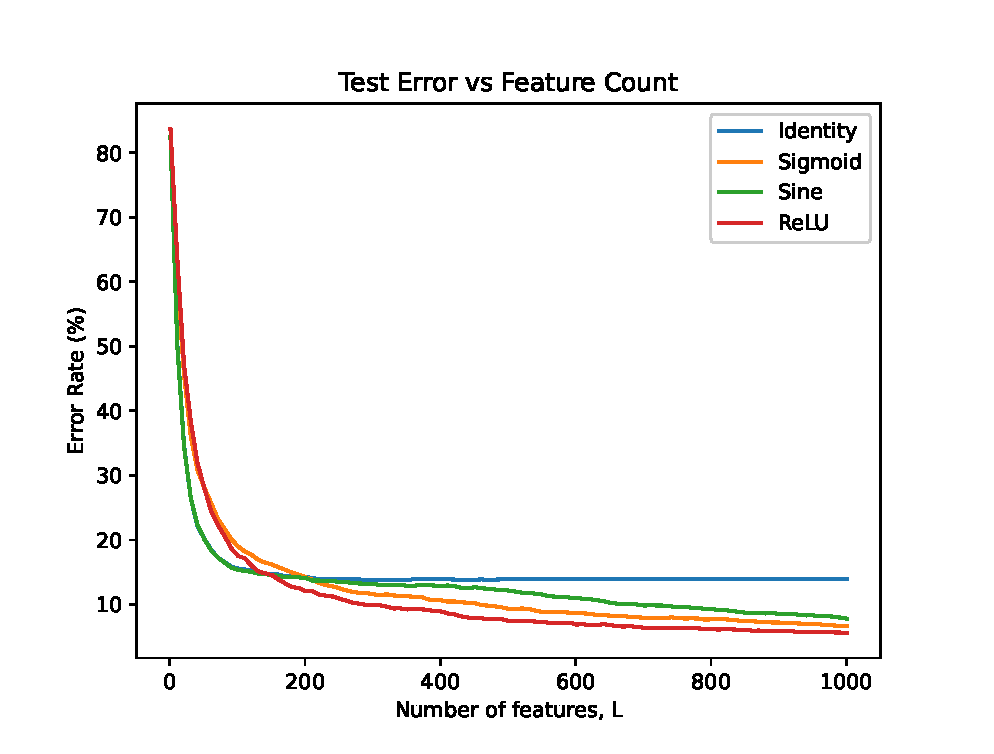
\includegraphics[width=\textwidth]{images/one_vs_all_test_error_vs_features.eps}
        \caption{Test error rate vs feature count}
    \end{minipage}
\end{figure}
I plotted 100 equally space values of $L$ from $1$ to $1001$.
We can clearly see that after a certain number of features, \textasciitilde170, the rate of decrease in error sharply decreases, and we see diminishing returns on accuracy.

\begin{table}
    \caption{Error Rates of Different Feature Mappings with One-Versus-One Classifier}
    \label{sample-table}
    \centering
    \begin{tabular}{l|ll}
      \toprule
      Mapping     & Training Error     & Test Error \\
      \midrule
      Identity & $14.23$\%  & $13.97$\%     \\
      Sigmoid     & $6.60$\% & $6.63$\%      \\
      Sinusoid     & $7.77$\%       & $7.80$\%  \\
      ReLU     & $5.47$\%       & $5.58$\%  \\
      \bottomrule
    \end{tabular}
  \end{table}
%----------------------------------------------------------------------------------------------------------------------------------------------------------------------------------------------
\subsection{One-Versus-One Classifier}
Similar to the one-versus-all classifier, I wrote some helper methods to assist in creating the models for each feature mapping.
\begin{lstlisting}
    def create_model(x, y, labels):
        model = np.empty((10,10, x.shape[1]))

        for i in range(len(labels)):
            for j in range(i+1, len(labels)):
                mask = ((y[:,0] == labels[i]) | (y[:,0] == labels[j]))
                filtered_Y = y[mask]
                filtered_X = x[mask]

                filtered_Y[filtered_Y == labels[j]] = -1
                filtered_Y[filtered_Y == labels[i]] = 1
                model_ij = np.matmul(np.matmul(np.linalg.pinv(np.matmul(filtered_X.transpose(),filtered_X)),filtered_X.transpose()),filtered_Y)
                model[i,j,:] = model_ij[:,0]
        return model

    def create_model_error_analysis(trueY, predictions):
        error = 0
        for i in range(len(predictions)):
            if(predictions[i] != trueY[i]):
                error = error + 1
        error = (error / len(trueY)) * 100
        return error
    def predict_one_vs_one(x, model, labels):
        votes = np.zeros((x.shape[0], labels.shape[0]))
        for i in range(len(labels)):
            for j in range(i+1, len(labels)):
                prediction_ij = np.matmul(x, model[i,j,:])
                votes[prediction_ij > 0,i] = votes[prediction_ij > 0,i] + 1
                votes[prediction_ij < 0,j] = votes[prediction_ij < 0,j] + 1
        predictions = np.argmax(votes, axis=1)
        return predictions
    def plot_confusion_matrix(trueY, predictions, labels, colors, feature_type, data_type):
        display=metrics.ConfusionMatrixDisplay.from_predictions(trueY, predictions,labels=labels, cmap=colors)
        plt.title(f'Error: {create_model_error_analysis(trueY, predictions):.2f}%')
        display.figure_.savefig(f'/Users/pranavreddy/Desktop/ECE 174/Project1/images/one_vs_one_{data_type.lower()}_confusion_matrix_{feature_type}.eps')
        plt.show()
\end{lstlisting}

\newpage
\FloatBarrier
\subsubsection{Identity Feature Mapping}
\begin{figure}[h!]
    \centering
    \begin{minipage}{0.5\textwidth}
        \centering
        \includegraphics[width=\textwidth]{images/one_vs_one_training_confusion_matrix_Identity.eps}
        \caption{Confusion matrix for training data.}
    \end{minipage}\hfill
    \begin{minipage}{0.5\textwidth}
        \centering
        \includegraphics[width=\textwidth]{images/one_vs_one_test_confusion_matrix_Identity.eps}
        \caption{Confusion matrix for test data.}
    \end{minipage}
\end{figure}
We can see that the identity feature mapping produces similar results to the one-versus-one classifier without the randomization.
These results are subject to some fluctuations due to the non-deterministic nature of the mapping.

\FloatBarrier
\subsubsection{Sigmoid Feature Mapping}
\begin{figure}[h!]
    \centering
    \begin{minipage}{0.5\textwidth}
        \centering
        \includegraphics[width=\textwidth]{images/one_vs_one_training_confusion_matrix_Sigmoid.eps}
        \caption{Confusion matrix for training data.}
    \end{minipage}\hfill
    \begin{minipage}{0.5\textwidth}
        \centering
        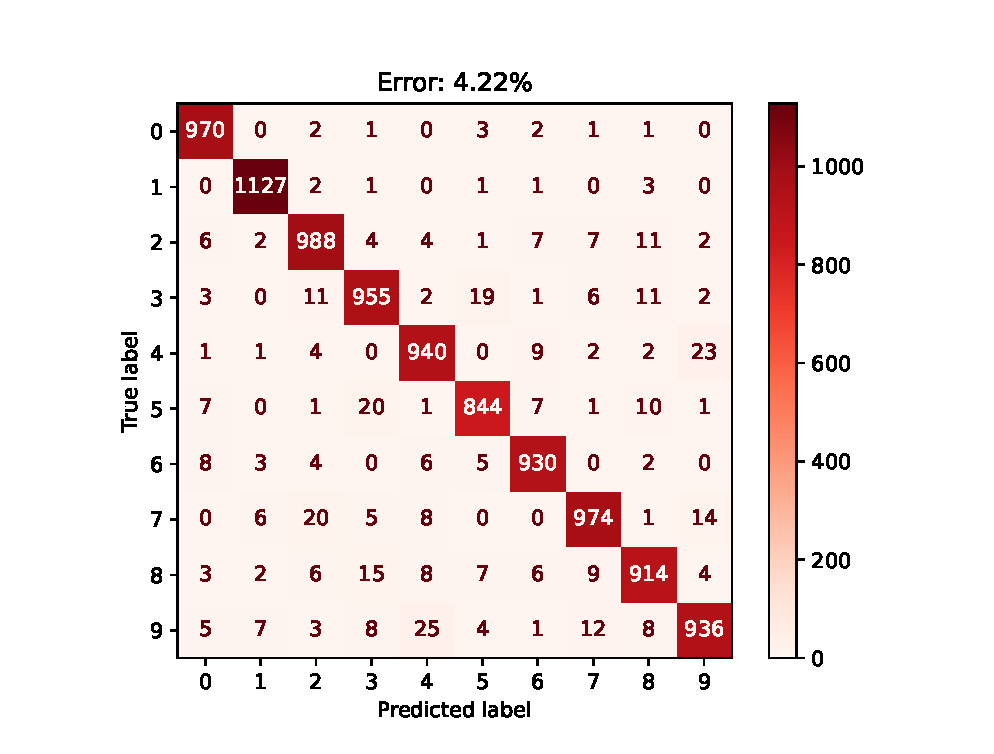
\includegraphics[width=\textwidth]{images/one_vs_one_test_confusion_matrix_Sigmoid.eps}
        \caption{Confusion matrix for test data.}
    \end{minipage}
\end{figure}
The sigmoid feature mapping produces better results than the one-versus-one model without the feature mapping, although the same digit pairs (3-5, 2-7, 4-9) producee significant error.
The generalization from the training data to test data is worse, as the increase in error is more than the other three feature mappings.

\FloatBarrier
\subsubsection{Sinusoid Feature Mapping}
\begin{figure}[h!]
    \centering
    \begin{minipage}{0.5\textwidth}
        \centering
        \includegraphics[width=\textwidth]{images/one_vs_one_training_confusion_matrix_Sine.eps}
        \caption{Confusion matrix for training data.}
    \end{minipage}\hfill
    \begin{minipage}{0.5\textwidth}
        \centering
        \includegraphics[width=\textwidth]{images/one_vs_one_test_confusion_matrix_Sine.eps}
        \caption{Confusion matrix for test data.}
    \end{minipage}
\end{figure}
Once again, the same pairs produce error, but the increase in error from the training data to the test data is not as sharp as the increase for sigmoid, but it is more than the ReLU.

\FloatBarrier
\subsubsection{Recitfied Linear Unit (ReLU) Feature Mapping}
\begin{figure}[h!]
    \centering
    \begin{minipage}{0.5\textwidth}
        \centering
        \includegraphics[width=\textwidth]{images/one_vs_one_training_confusion_matrix_ReLU.eps}
        \caption{Confusion matrix for training data.}
    \end{minipage}\hfill
    \begin{minipage}{0.5\textwidth}
        \centering
        \includegraphics[width=\textwidth]{images/one_vs_one_test_confusion_matrix_ReLU.eps}
        \caption{Confusion matrix for test data.}
    \end{minipage}
\end{figure}
The ReLU dataset still has the same error-prone pairs of numbers, but it performs the best out of all the feature mappings, and also has the least increase in error from training to test.

\FloatBarrier
\subsubsection{Effect of Features on Performance of One-Versus-One Classifier}
\begin{figure}[h!]
    \centering
    \begin{minipage}{0.5\textwidth}
        \centering
        \includegraphics[width=\textwidth]{images/one_vs_one_training_error_vs_features.eps}
        \caption{Training error rate vs feature count.}
    \end{minipage}\hfill
    \begin{minipage}{0.5\textwidth}
        \centering
        \includegraphics[width=\textwidth]{images/one_vs_one_test_error_vs_features.eps}
        \caption{Test error rate vs feature count}
    \end{minipage}
\end{figure}
For the sake of time, I only plotted 10 equally space values of $L$ from $1$ to $1001$.
We can clearly see that after a certain number of features, \textasciitilde170, the rate of decrease in error sharply decreases, and we see diminishing returns on accuracy.

\begin{table}
    \caption{Error Rates of Different Feature Mappings}
    \label{one-vs-one-mapping-errors}
    \centering
    \begin{tabular}{l|ll}
      \toprule
      Mapping     & Training Error     & Test Error \\
      \midrule
      Identity & $6.19$\%  & $6.99$\%     \\
      Sigmoid     & $2.88$\% & $4.22$\%      \\
      Sinusoid     & $3.04$\%       & $4.42$\%  \\
      ReLU     & $2.21$\%       & $3.56$\%  \\
      \bottomrule
    \end{tabular}
\end{table}

\nocite{*}
\bibliography{bibliography.bib}


\end{document}